% ANEXOS
\appendices

\section{Correcciones a la plantilla BER de la Fase 4}
\label{app:correcciones}
Los archivos originales se conservan sin cambios en \texttt{02\_GNU\_Radio/Archivos\_originales}; las versiones corregidas están en \texttt{Archivos\_modificados}. Al abrir la plantilla original en GRC~3.10.12, \texttt{e\_BER\_Curve} y ``Guardar curva BER en CSV'' se muestran con error (título en rojo) y \texttt{e\_BER\_Curve} no expone parámetros.

\begin{lstlisting}[style=bonito, language=Python, caption={Cambios en \texttt{e\_BER\_Curve} y \texttt{e\_BER\_CSV}}, label={lst:correcciones}]
# e_BER_Curve (original -> corregido)
class blk(gr.sync_decimator):          # no es bloque Python en GR 3.10
class blk(gr.decim_block):             # pasarela Python correcta
    gr.decim_block.__init__(self, name='e_BER_Curve', in_sig=[np.int8, np.int8],
        out_sig=[(np.float32, self.N), (np.float32, self.N)], decim=self.update_every)

# e_BER_CSV (original -> corregido)
self.carpeta = Path(__file__).resolve().parent
try:
    self.carpeta = Path(__file__).resolve().parent
except NameError:   # GRC instancia el bloque sin __file__ al validarlo
    self.carpeta = Path.cwd()
\end{lstlisting}

\section{Evidencias de ejecución en el equipo del grupo}
\label{app:evidencias}
La Figura~\ref{fig:gui_pc} es una captura de pantalla real de la GUI de \texttt{S3\_Multitrayectoria\_BPSK\_Grupo5.grc} ejecutándose en GNU Radio Companion 3.10.12 (radioconda, Windows) con la prueba C seleccionada. La Figura~\ref{fig:grc_ber} muestra el flujograma con la instrumentación BER integrada.

\begin{figure}[!h]
\centering
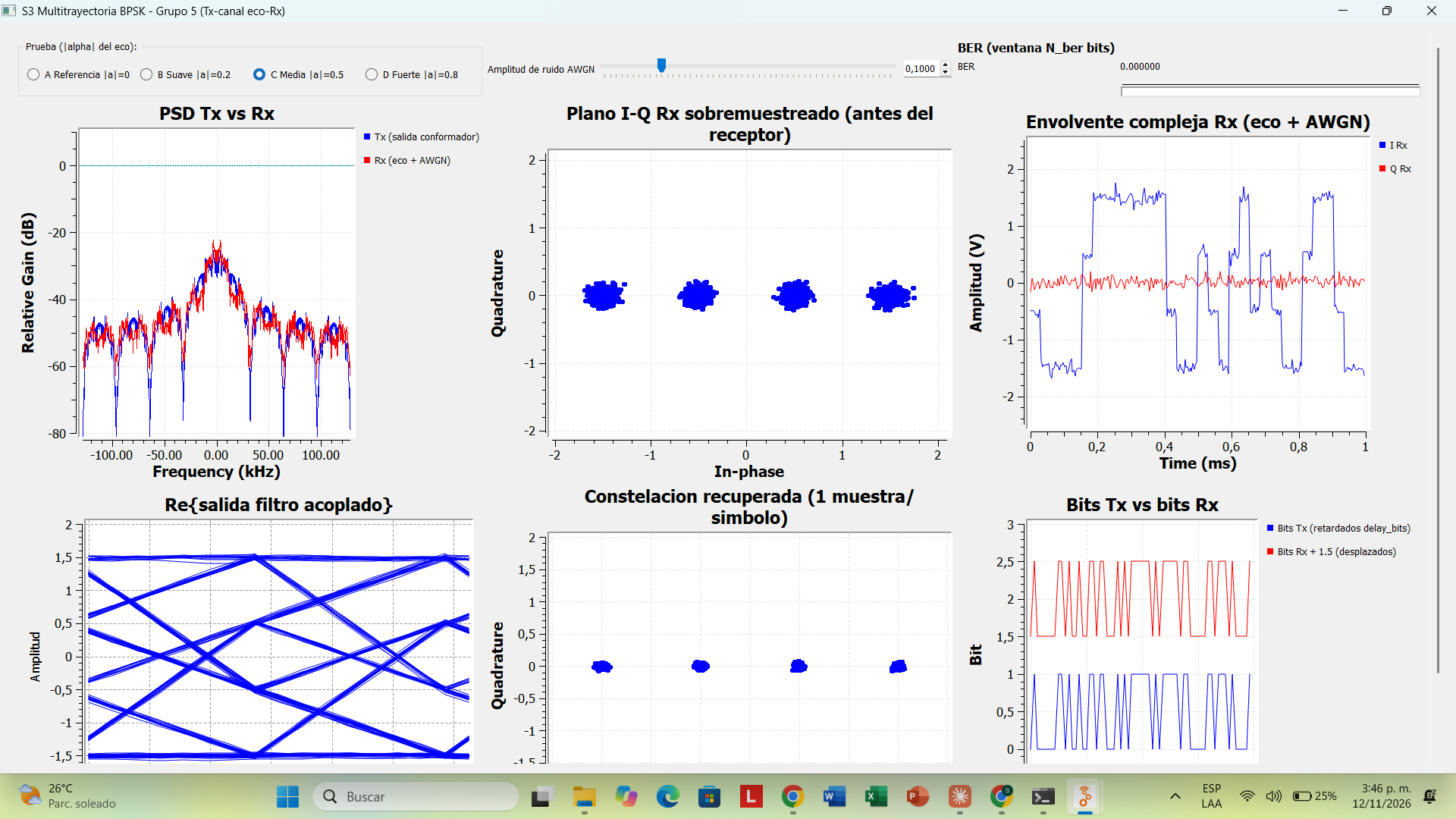
\includegraphics[width=\columnwidth]{PC_GUI_ejecucion_Prueba_C_media.jpg}
\caption{GUI en ejecución (prueba C): PSD Tx/Rx, plano I-Q, envolvente, ojo, constelación recuperada, bits Tx/Rx y medidor de BER.}
\label{fig:gui_pc}
\end{figure}

\begin{figure}[!h]
\centering
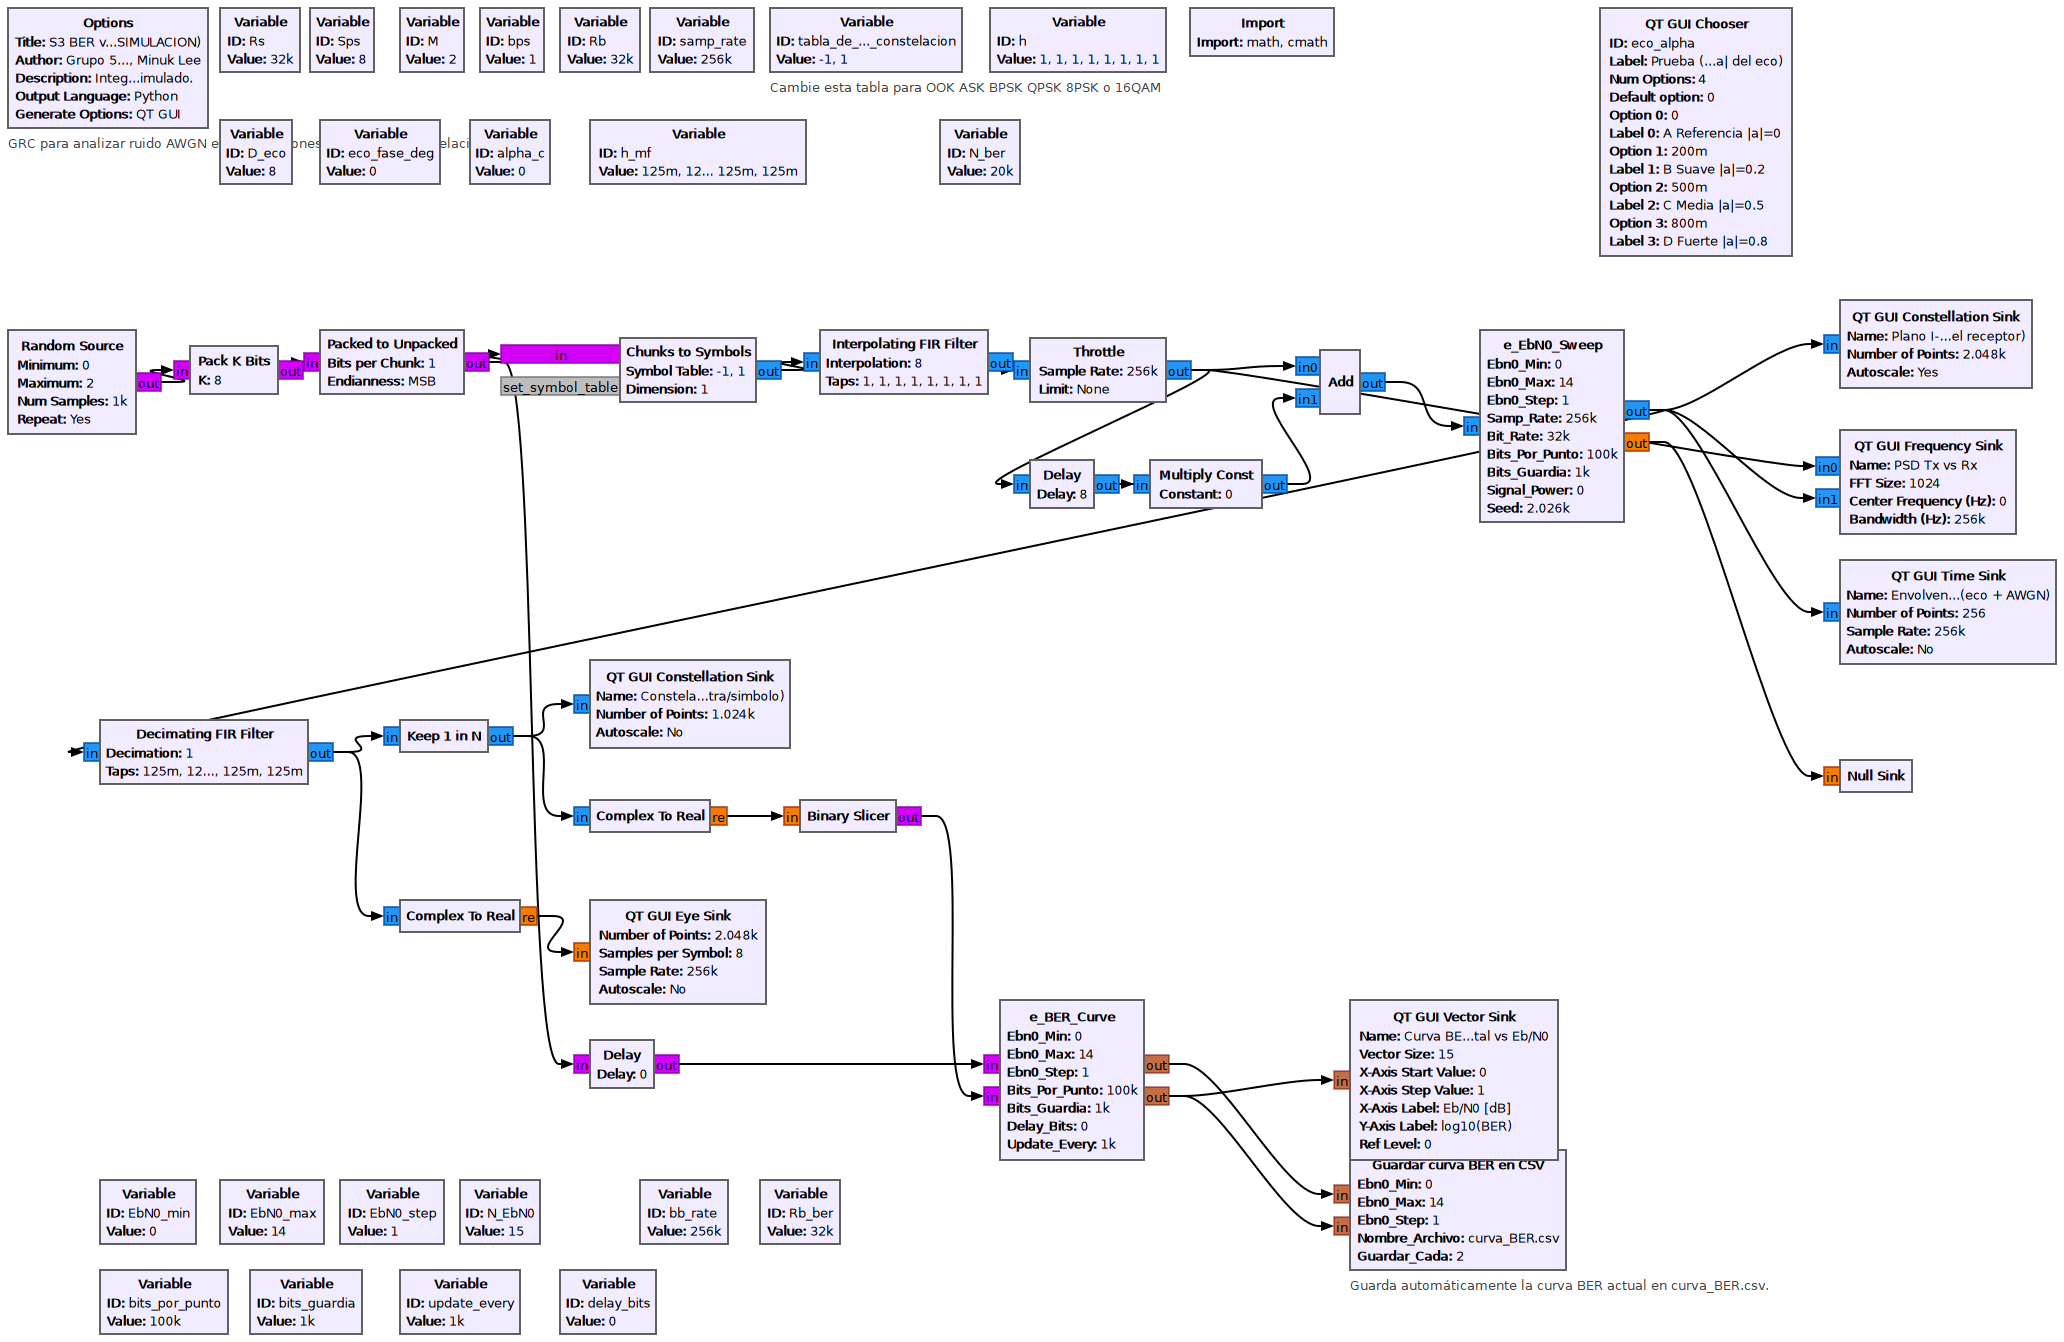
\includegraphics[width=\columnwidth]{GRC_S3_BER_Multitrayectoria_BPSK_Grupo5.png}
\caption{\texttt{S3\_BER\_Multitrayectoria\_BPSK\_Grupo5.grc}: \texttt{e\_EbN0\_Sweep} antes del receptor, y \texttt{e\_BER\_Curve} con la referencia Tx y los bits Rx.}
\label{fig:grc_ber}
\end{figure}

\section{Uso de herramientas de IA}
Se utilizó un asistente de IA (Claude, de Anthropic) para organizar el trabajo, generar los flujogramas a partir de los archivos del curso, automatizar la exportación de datos y las gráficas y proponer borradores de redacción. Todas las cifras provienen de ejecuciones de GNU Radio (3.10.9 en Linux y 3.10.12 en el equipo del grupo) y se contrastaron con la teoría. Las decisiones y conclusiones deben ser revisadas y asumidas por los integrantes del Grupo~5 antes de la entrega.
